\documentclass[12pt]{iopart}
\usepackage{iopams}
\usepackage{graphicx}
\usepackage{enumerate}
\begin{document}
\article[Optimal design for fitting experimental data]{TECHNICAL DESIGN NOTE}{Optimal design for fitting experimental data}
%%\author{G Imreh and W-Y Cheng}
\address{Institute of Atomic and Molecular Sciences, Academia Sinica, Taiwan}
%%\ead{\mailto{imrehg@gmail.com}}
\begin{abstract}
Optimal design methodology for spectroscopy and other fitted things.
\end{abstract}

\noindent{\it Keywords\/}:

\pacs{}
%%\submitto{\MST}

%%%%%%%%%%%%%%%%%%%%%%%%%%%%%%%%%%%%%% Theory

\section{Introduction}

Experiments are not limited to the physical sciences, but many areas of science, even industry makes use of them: a process is described by a mathematical model and repeated observations are used to evaluate the model and estimate its free parameters. When designing an experiment, the most common aims are the ability to estimate the model parameters without bias and as well as possible, ability to detect lack of fit, and to use the fewest number of observations \cite{Box1975,Box1987}. The last aim is often considered secondary in physical experiments, however as this note will show, the three aims are interconnected.

The possible input parameters for an experiment form the $\mathcal{X}$ design region. From $\mathcal{X}$ one chooses $N$ points $x_i$, $i = 1, \ldots, N$ to conduct the experiment. Using optimal experimental design (OED) theory, with different choices of $x_i$ one can adjust the experiment towards different goals: overall best estimate of the model parameters, best estimate (smallest variance) of a subset of important parameters at the expense of others, best estimate of a function of the model parameters, most sensitive lack-of-fit measure. The list is by no means exhaustive, but represent the most common cases in physics experiments. Most researchers spread the observations uniformly in the region of interest, which is often sub-optimal in all criteria. OED is a rich area of statistics, mostly used in medical research and industrial quality control, mainly due to those fields close connection to statistics, not because of the lack relevance to other fields. There were previous efforts to use OED for physics, such as optimal measurement of processes described by differential equations, e.g. the placement of temperature sensors in heat conductivity experiments \cite{Emery1998}. This note hopes to introduce the methodology of OED for model parameter estimation (fitting), examine its suitability for physical experiments and give examples to help implementation.


\section{Optimal design}
Short introduction of linear regression using matrix algebra, only to show the notation in this paper. For more detailed explanation check any standard linear algebra text book. Measure $y_i$ at $x_i$ points ($i=1, \ldots, N$)
\begin{equation}
E[Y] = F \beta
\end{equation}
where $Y$ is the $N \times 1$ vector of responses, $\beta$ is a $p \times 1$ vector of unknown parameters, and $F$ is the $N \times p$ extended design matrix. The $i$th row of $F$ is $f^T(x_i)$, a known function of the $m$ explanatory variables. As an example, for the model $y = \beta_1 + \beta_2 x_1 + \beta_3 x_1 x_2 + \beta_4 x_2^2$ the information matrix has rows of
\begin{equation}
f^T(x_i) = \left[
	\begin{array}{c c c c}
	1 & x_{1i} & x_{1i}x_{2i} & x_{2i}^2.
	\end{array}\right]
\end{equation}
For this model $m = 2$ and $p = 4$.



Least squares linear regression is then written as:
\begin{equation}
\hat \beta = (F^T F)^{-1} F^T y
\end{equation}
The covariance matrix of the least squares estimates is
\begin{equation}
\mathrm{var} \hat \beta = \sigma^2 (F^T F)^{-1}
\label{eq:varbeta}
\end{equation}
where $\sigma$ is the error variance. The errors are assumed to be normally distributed with 0 mean. The predicted value of the function is
\begin{equation}
\hat y(x) = f^T(x) \hat \beta
\end{equation}
with variance
\begin{equation}
\mathrm{var}\{\hat y(x)\} = \sigma^2 f^T(x)\left(F^T F\right)^{-1}f(x).
\end{equation}
Optimal design then stems from the question: which are the best $x_i$ points to measure to minimize the variance of the model parameters? The answer to this question also points the the way to optimize $x_i$ for other goals as well.


\subsection{Optimal design}
Without a loss of generality we can assume the explanatory variable $x$ as one-dimensional. 
Let's define the continuous design function $\xi$ as a measure over the design region $\mathcal{X}$. If $\xi$ has $n$ distinct support points, then
\begin{equation}
\xi = \left\{
  \begin{array}{l l l l}
    x_1 & x_2 & \ldots & x_n\\
    w_1 & w_2 & \ldots & w_n\\
  \end{array} \right \}
\end{equation}
where $w_i$ is the weight of point $x_i$, $\int_{\mathcal{X}}\xi(dx) = 1$ and $0 \leq w_i \leq 1$ for every $i$, which in our problem setting means to conduct the experiment at $x_i$ in $w_i$ fraction of the time.

For clarity, $\xi$ can also be rewritten with delta-functions as
\begin{equation}
\xi(x) = \sum_i w_i \delta(x - x_i).
\label{eq:xidelta}
\end{equation}

Exact design is finite version of $\xi$ for realizable integers $r_i$ for a total number of $N = \sum_i r_i$ trials:
\begin{equation}
\xi_N = \left\{
  \begin{array}{l l l l}
    x_1 & x_2 & \ldots & x_n\\
    r_1/N & r_2/N & \ldots & r_n/N\\
  \end{array} \right \}
\end{equation}
The information matrix will depend on the design function as
\begin{equation}
M(\xi) = \int_{\mathcal{X}} f(x)f^T(x) \xi(dx) = \sum_{i=1}^n f(x_i)f^T(x_i)w_i
\label{eq:infcont}
\end{equation}
summing over the $n$ design points.
The N-trial exact design
\begin{equation}
F^T F = \sum_{i=1}^N f(x_i) f(x_i)^T
\end{equation}
which has to be scaled to get the information matrix of
\begin{equation}
M(\xi_N) = \frac{F^T F}{N}
\end{equation}
The variance of the response is given by
\begin{equation}
\mathrm{var}\{\hat y(x)\} = \sigma^2 f^T(x) M^{-1}(\xi) f(x)
\end{equation}
from where the standardized variance of the predicted response is
\begin{equation}
d(x, \xi) = f^T(x) M^{-1}(\xi) f(x)
\label{eq:stdvar}
\end{equation}
that is function of both $x$ where the prediction is made and the design $\xi$.
For an exact design
\begin{equation}
d(x, \xi_N) = f^T(x) M^{-1}(\xi_N) f(x) = \frac{N \mathrm{var}\{\hat y(x)\}}{\sigma^2}
\end{equation}

Looking at the variance of the fitted model parameters as shown in \eref{eq:varbeta}, it depends on the inverse of the information matrix $M = F^TF$. The best prediction is achieved when $M^{-1}$ is minimal, which is equivalent to maximum of $M$. In general $\beta$ is a vector, thus one wants to maximize the determinant $|M|$ for the overal best prediction. This is the so--called $D$-optimal design (as ``determinant'').

\subsection{Requirements of the optimum}
\label{sec:get}

In the theory of continuous designs one considers the minimization of a general function of imprecision $\Psi\{M(\xi)\}$. Under the mild requirements of compact $\mathcal{X}$, convex and differentiable $\Psi$ it can be shown that $\xi$ that minimizes $\Psi$ also satisfies a number of other conditions. For example in the case of $D$-optimality the determinant of the information matrix is maximized, thus
\begin{equation}
\Psi\{M(\xi)\} = \log|M^{-1}(\xi)| = - \log|M(\xi)|.
\end{equation}
The General Equivalence Theorem is then an application of the fact that the derivatives of a function are zero at its minimum. In our case $\Psi$ depends on the measure $\xi$ through the information matrix. Let $\bar \xi$ put unit mass at a point $x$ and a new measure $\xi'$ be given by
\begin{equation}
\xi' = (1-\alpha)\xi + \alpha \bar \xi
\end{equation}
\Eref{eq:infcont} shows that the information matrix is additive, thus
\begin{equation}
M(\xi') = (1-\alpha)M(\xi) + \alpha M(\bar \xi).
\end{equation}
The derivative of $\Psi$ is then
\begin{equation}
\phi(x, \xi) = \lim_{\alpha \rightarrow 0^+} \frac{1}{\alpha}\left[\Psi\{(1-\alpha)M(\xi) + \alpha M(\bar \xi)\} - \Psi\{M(\xi)\}\right]
\label{eq:deriv}
\end{equation}
The General Equivalence Theorem then states that the conditions
\begin{enumerate}[(a)]
\item the design $\xi^*$ minimizes $\Psi\{M(\xi)\}$
\item the minimum of $\phi(x, \xi^*) \geq 0$
\item $\phi(x, \xi^*)$ achieves minimum at the support points of the design
\end{enumerate}
are equivalent. This result can be directly used to find the optimal design $\xi^*$ under various optimality conditions.

For example in case of $D$-optimality it can be shown that the derivative function \eref{eq:deriv} is
\begin{equation}
\phi(x, \xi) = p - d(x, \xi)
\label{eq:phicond}
\end{equation}
where $d(x, \xi)$ is the standardized variance defined in \eref{eq:stdvar}. From condition (a) above the optimal design $\xi^*$ has
\begin{equation}
d(x, \xi^*) \leq p
\end{equation}
with equivalence at the support points.

\subsection{Finding the optimal design}

The General Equivalence Theorem implies that away from the optimum $\phi(x, \xi) < 0$. Then we can choose the measure $\bar \xi_k$ that puts onit mass at point $x_k$ as $\phi(x_k, \xi_k) < 0$, then
\begin{equation}
\xi_{k+1} = (1-\alpha_k) \xi_k + \alpha \bar \xi_k
\end{equation}
will lead to decrease in $\Psi$ if $\alpha_k$ is small enough. The above describes a family of descent algorithms. The best convergence can be achieved if $x_k$ chosen as $\phi(x_k, \xi_k)$ has a minimum. In the original construction of these algorithms $\alpha_k = (k+1)^{-1}$ was chosen.

According to \eref{eq:phicond}, in the case of $D$-optimal design, the $x_k$ that minimizes $\phi(x_k, \xi_k)$ will maximize $d(x_k, \xi_k)$. Knowing $f^T(x)$ and thus $M$, one can analytically optimize $|M|$, however that route is only possible in the simplest cases. For most models a numerical optimization routine is needed. Most numerical methods are based on points added to or removed from a candidate design measure. One of the simplest, frequently used sequential method to generate $\xi^*$ in practice is the following:
\begin{enumerate}
\item choose $n$ arbitrary starting points that have a non-singular information matrix, thus defining $\xi_n$ with equal weights.
\item calculate $x_{n+1} = \mathrm{argmax}\left\{d(x, \xi_n)\right\}$ for $x \in \mathcal{X}$ and add it to the design.
\item repeat until algorithm converges, that is when $\max_{x} d(x, \xi_{n}) \approx p$.
\item throw away sub-optimal starting points
\item the distribution of $x_i$ will suggest the of the optimal measure $\xi^*$
\end{enumerate}
There are other numerical methods fidning $\xi^*$, however in practice the one above is the most straightforward to implement and interpret.

Regardless of the optimization method, the provisional $xi^*$ should be verified by checking that $d(x, \xi_{n}) \lesssim p$ over the whole $\mathcal{X}$. Also, it can be shown that if $\mathcal{X} = \mathbb{R}^m$ then $\xi^*$ has $p$ support points with equal weights. If $\mathcal{X} \subsetneq \mathbb{R}^m$ then $n \geq p$, which might have unequal weights.

The relative efficiency of two $D$-optimal designs $\xi_1$ and $x_2$ is defined as
\begin{equation}
D_\mathrm{eff} = \left\{\frac{|M(\xi_1)|}{|M(\xi_2)|}\right\}^{1/p}
\end{equation}
which is an efficiency measure independent of the $p$ dimension of the model. Because of the additivity of the information matrix, the meaning of the relative efficiency is that to provide the same tightness of model parameter estimates, $\xi_2$ requires $D_\mathrm{eff}$ number of trials compared to $\xi_1$. For example in case of $D_\mathrm{eff} = 0.5$ an experiment using $\xi_1$ would require twice as many trials as $\xi_2$.

An advantage of the $D$-optimality is that the optimum measure $\xi^*$ does not depend on the scale of the explanatory variables. Linear transformations leave the $D$-optimum design unchanged.


\subsection{Optimize for a subset of parameters}

In case one wants to estimate an $s < p$ subset of model parameters more precisely than rest, the information matrix can be partitioned as
\begin{equation}
M(\xi) = \left[
  \begin{array}{l l}
    M_{11}(\xi)   & M_{12}(\xi)\\
    M^T_{12}(\xi) & M_{22}(\xi)
  \end{array} \right]
\end{equation}
where $M_{11}(\xi)$ is the $s \times s$ upper sub-matrix of the information matrix. Then the $M^{11}(\xi)$, the $s \times s$ upper sub-matrix of the inverse will be
\begin{equation}
M^{11}(\xi) = \left\{M_{11}(\xi) - M_{12}(\xi)M^{-1}_{22}(\xi)M^T_{12}(\xi)\right\}^{-1}
\end{equation}
and the $D_s$ design optimizes for 
\begin{equation}
|M_{11}(\xi) - M_{12}(\xi)M^{-1}_{22}(\xi)M^T_{12}(\xi)| = \frac{|M(\xi)|}{|M_{22}(\xi)|}.
\end{equation}
This expression gives the standardized variance as
\begin{equation}
d_s(x, \xi) = f^T(x) M^{-1}(\xi)f(x) - f_2^T(x) M_{22}^{-1}(\xi)f_2(x)
\label{eq:dsvar}
\end{equation}
with optimality requirement of
\begin{equation}
d_s(x, \xi^*) \leq s
\end{equation}
and efficiency
\begin{equation}
D_\mathrm{eff} = \left\{\frac{|M(\xi_1)|/|M_{22}(\xi_1)|}{|M(\xi_2)|/|M_{22}(\xi_2)|}\right\}^{1/s}
\end{equation}

One potential difficulty with $D_s$-optimality, that $M(\xi^*)$ can turn out to be singular. In that case numerical regularization can avoid the problem, that is adding a small multiple of the identity matrix as
\begin{equation}
M_\epsilon(\xi) = M(\xi)  + \epsilon I
\end{equation}  
where $\epsilon$ is small, but large enough to be able to invert $M_\epsilon$ (in practice of the order of $10^{-5}$).

\subsection{Non-linear models and robustness}

Non-linear models cannot be expressed in the previous matrix formalism, but can be linearised to be able to use optimal design methods. If $\eta(x, \theta)$ is a non-linear function of $x$ with parameter $\theta$, Taylor expansion at the parameter estimate yields
\begin{equation}
E[Y] = \eta(x, \theta) = \eta(x, \hat \theta) + (\theta - \hat \theta) \frac{\partial \eta}{\partial \theta}(x, \theta)|(\theta = \hat \theta) + \ldots
\end{equation}
or rewritten to emphasise the linear model
\begin{equation}
E[Y] - \eta(x, \hat \theta) = \beta f(x)
\end{equation}
where $\beta = \theta - \hat \theta$. It is straightforward to extend the linearization to vector-parameters and to higher order Taylor-terms if needed.

A complication with non-linear models is that many times the information matrix $F(x)$ will be also a function of the parameter $\hat \theta$, thus the optimal design $\xi$ is truly optimal only for a given set of parameters. One then have to evaulate the robustness of the parameter estimation for a given model and $\xi$ by calculating the change in $D_\mathrm{eff}$ as a function of the misspecified model parameters. 

If more robustness is required, we can still follow the optimal design-ideas to to keep some of the efficiency gains. Consider the delta function expression of $\xi$, given in \eref{eq:xidelta}. The delta function can be considered as a limiting version of a finite distribution, such as
\begin{equation}
\delta(x) = \lim_{\epsilon \rightarrow 0} \frac{1}{\sqrt{2 \pi} \epsilon } \exp\left(-\frac{x^2}{2 \epsilon^2}\right).
\end{equation}
Using a finite $\epsilon$ in the measure $\xi$ while keeping the original support points can improve robustness. \Sref{seq:exopt} and \sref{seq:exopts} contains examples of such calculation, and show that $D$-optimality can be quite robust, while $D_s$-optimality is less so.

\subsection{Non-uniform error variance}

Some physical measurements are known to have non-uniform error variance as a function of the response variable $y$, e.g. photon counting which has a Poissonian distribution, thus the variance of $y_i$ is approximately $\sqrt{y_i}$ instead of a independent of $y_i$. In a general case let the variance of an observation at $x_i$ be $\sigma^2/w(x_i)$ where $w(x_i)$ are a set of known weights. If $W = \mathrm{diag}\{w(x_i)\}$, then the weighted least squares estimate of $\beta$ is
\begin{equation}
\hat \beta = (F^T W F)^{-1} F^T W y
\end{equation}
with variance
\begin{equation}
\mathrm{var}(\hat \beta) = \sigma^2 (F^T W F)^{-1}.
\end{equation}
The information matrix of \eref{eq:infcont} can be rewritten as
\begin{equation}
M(\xi) = \int_{\mathcal{X}} w(x) f(x)f^T(x) \xi(dx)
\end{equation}
and the previous methods for the $D$-optimal design can be used.

%\subsection{Functions of variables}
%
%
%
%C-optimum design (as "constans"):
%
%\begin{equation}
%\mathrm{var}\left\{g(\hat \theta)\right\} = \mathrm{var}(c^T \hat \beta) = c^T M^{-1}(\xi) c
%\end{equation}
%where $c$ is a $p \times 1$ vector of known constans. Generally, it can be defined from the Tailor expansion:
%\begin{equation}
%c_i(\theta) = \frac{\partial g(\theta)}{\partial \theta_i}
%\end{equation}
%
%Have to be careful, though, because the model can be singular. For linear models this means maybe only linear combinations of parameters can be estimated, for nonlinear models it is possible that the parameter won't be observable. Care needed!


\subsection{Optimal model discrimination}

Optimal design methods can also be used to discriminate between competing models. Let's write the true model as $\eta_t(x)$. If a second model is fitted to the data, in absence of errors, its parameter estimates will be given by
\begin{equation}
\hat \theta_2(\xi) = \min_{\theta_2} \int_{\mathcal{X}} \left\{\eta_t(x) - \eta_2(x, \theta_2)\right\}^2 \xi(\mathrm{d}x)
\end{equation}
and the residual sum of squares (RSS) as
\begin{equation}
\Delta_2(\xi) = \int_{\mathcal{X}} \left\{\eta_t(x) - \eta_2(x, \hat \theta_2(\xi))\right\}^2 \xi(\mathrm{d}x)
\label{eq:rss}
\end{equation}
The design that maximises $\Delta_2{\xi}$ is called $T$-optimal (as ``test''). $T$-optimal designs thus aim at producing the largest RSS for the fewest number of trials. To generate the $T$-optimal $\xi^*$ we can use the General Equivalence Theorem laid out in \sref{sec:get}. The maximization $\Delta_2{\xi}$ is done by the help of its derivative
\begin{equation}
\psi_2(x, \xi) = \left\{\eta_t(x) - \eta_2(x, \hat \theta_2(\xi))\right\}^2
\end{equation}
and thus for $T$-optimal design $\xi^*$: $\psi_2(x, \xi^*) \leq \Delta_2(\xi^*)$ for $x \in \mathcal{X}$, with equivalence at the support points. For any non-optimal design, that is $\Delta_2(\xi) < \Delta_2(\xi)$, it will also be $\sup_{x \in \mathcal{X}} \psi_2(x, \xi) > \Delta_2(\xi^*)$.

We can then follow a very similar route to generate $\xi^*$ for any two models $\eta_1(x, \theta_1)$ and $\eta_2(x, \theta_2)$. Without a loss of generality, we can assume that the true model is $\eta_1$. Then
\begin{enumerate}[(a)]
\item if there are $p$ different parameters altogether in the two models, choose $n = p+1$ separate points in the design region ($\xi_n$)
\item calculate the value of $\eta_1$ for these points and true parameter $\theta_1$, and get the best fit parameter value $\theta_2$ for the second function
\item find $x_{n+1} = \mathrm{argmax}_{x \in \mathcal{X}}\psi_2(x, \xi_n) = \mathrm{argmax}_{x \in \mathcal{X}} \left\{\eta_1(x, \theta_1) - \eta_2(x, \hat \theta_2(\xi_n))\right\}^2$ and add to the design
\item repeat until algorithm converges, remove the sub-optimal starting points and the remainder should suggest $\xi^*$.
\end{enumerate}

In practice, however, one seldom knows in advance which model will be correct. The the algorithm can be modified. Take a $k$ number of measurements and obtain parameter estimates of $\hat \theta_{1k}$ and $\hat \theta_{2k}$. The derivative function is then $\psi_2(x, \xi_k) = \left\{\eta_1(x, \theta_1) - \eta_2(x, \hat \theta_2(\xi_n))\right\}^2$. Find $x_{k+1}$ for which $\psi(x_{k+1}, \xi_k) = \sup_{x \in \mathcal{X}}\psi_2(x, \xi_n)$. The $(k+1)$th observation is than taken at $x_{k+1}$. As $k \rightarrow \infty$ one of the models converge to the true model, then this method will converge to the $T$-optimal design. Repeat until suitable precision is achieved.

If one has a value of $\Delta_2(\xi^*)$ and the error variance $\sigma^2$, it is possible to get an estimate of the $N$ required number of trials for any given precision. If we include the error variance in the \eref{eq:rss} expression of RSS it will be
\begin{equation}
\Delta_2(\xi^*, \sigma) = \int_{\mathcal{X}} \left[\left\{\eta_t(x) - \eta_2(x, \hat \theta_2(\xi^*))\right\}^2 + \sigma^2\right]\xi(\mathrm{d}x).
\label{eq:rssvar}
\end{equation}
For linear models and large $N$ the RSS will have a non-central $\chi^2$ distribution, with non-centrality parameter
\begin{equation}
\frac{N\Delta_2(\xi^*, \sigma)}{\sigma^2 } = \frac{N \Delta_2(\xi^*)}{\sigma^2} + N
\end{equation}
and degrees of freedom of $df = N - p - 1$. Then using $\chi^2$ tables or built in functions in most mathematical software package, one can find $N$ that will have better than a pre-set $\alpha$ probability that the $\chi^2$ distribution is non-central (i.e. the given model can be rejected).


%%%%%%%%%%%%%%%%%%%%%%%%%%%%%%%%%%%%%% Practice

\section{Example: Lorentzian spectral line}

\subsection{3-parameter unrestricted model}
\label{seq:exopt}

The following examples of optimal design are based on spectroscopic experiments, but should be general enough to provide guidance for any other models.

In this hypothetical experiment we are trying to measure an atomic fluorescence lineshape of simple system, a Lorentzian function of the excitation light frequency:
\begin{equation}
\eta(x) = I \frac{\Gamma}{(x - x_0)^2 + \Gamma^2}
\label{eq:lorentz3}
\end{equation}
where $I$ is the height of the peak, $x_0$ is the centre frequency and $\Gamma$ is the half-with at half maximum. The partial derivatives for the Taylor-expanson are
\begin{eqnarray}
\frac{\partial \eta(x)}{\partial x_0} &=& I \frac{2 \Gamma (x - x_0)}{\left[(x - x_0)^2 + \Gamma^2\right]^2} \\
\frac{\partial \eta(x)}{\partial \Gamma} &=& I \frac{(x - x_0)^2 - \Gamma^2}{\left[(x - x_0)^2 + \Gamma^2\right]^2} \\
\frac{\partial \eta(x)}{\partial I} &=& \frac{\Gamma}{(x - x_0)^2 + \Gamma^2}
\end{eqnarray}
from which, our linearized model will be
\begin{equation}
E[y] = \eta(x) + (x_0 - \hat x_0) \frac{\partial \eta(x)}{\partial x_0} + (\Gamma - \hat \Gamma) \frac{\partial \eta(x)}{\partial \Gamma} + (I - \hat I) \frac{\partial \eta(x)}{\partial I}
\end{equation}
that can be reorganized as
\begin{eqnarray}
E[y] - \eta(x) &=& (x_0 - \hat x_0) \frac{\partial \eta(x)}{\partial x_0} + (\Gamma - \hat \Gamma) \frac{\partial \eta(x)}{\partial \Gamma} + (I - \hat I) \frac{\partial \eta(x)}{\partial I}  \nonumber \\
E[Y] &=& \beta F
\end{eqnarray}
where the coefficients are
\begin{equation}
\beta = \left[
  \begin{array}{l}
    x_0 - \hat x_0 \\
    \Gamma - \hat \Gamma\\
    I - \hat I \\
  \end{array} \right ]
\end{equation}
 and the $i$th row of $F$ is
\begin{equation}
 f^T(x_i) = \left[
  \begin{array}{l l l}
   \frac{\partial \eta(x_i)}{\partial x_0} & \frac{\partial \eta(x_i)}{\partial \Gamma} & \frac{\partial \eta(x_i)}{\partial I}
  \end{array} \right ]
\end{equation}
Without loss of generalization we can set $\hat x_0 = 0$, $\hat \Gamma = 1$, $\hat I = 1$, since the $x$ and $y$ range can always be rescaled to these values. Then we can look for the optimal design in the form of
\begin{equation}
\xi = \left\{
  \begin{array}{c c c}
    -a & 0 & a\\
    \frac{1}{3} & \frac{1}{3} & \frac{1}{3}\\
  \end{array} \right \}
\end{equation}
since our original function is symmetric with respect to 0 (hence $-a$ and $a$) and $\mathcal{X}~=~\mathbb{R}$ (thus the number of design points equal the dimension of $\beta$, with equal weights). Under these considetations we can calculate the information matrix $M$ as in \eref{eq:infcont}. The maximum of the determinat is found by differentiating with respect to $a$ and finding the roots. The calculation is straightforward but lengthy, thus we only quote the result of $a~\approx~0.7746$. This analytical method can cumbersome except for the simplest models (even with the available symbolic mathematic software). On the other hand, the sequential method of finding the correct parameters is much less intensive computationally. Let's start with a design of $x = [-1, 0, 1]$ which is still symetric and equal probability, but this is just to speed up the convergence of the algorithm. Any other $n \geq 3$ number for which $M$ is not singular could be chosen as a starting point. Then the sequential algorithms will create the following set of design points:
\begin{equation}
    -1, 0, 1, 0.577, -0.577, 0, -0.789,\ldots,0,-0.775,0.775,\ldots
\end{equation}
where the final ``$\ldots$'' just repeats the $0,-0.775,0.775$ sequence. We can then ignore the starting values and conclude that are design should be
\begin{equation}
\xi = \left\{
  \begin{array}{c c c}
    -0.775 & 0 & 0.775\\
    \frac{1}{3} & \frac{1}{3} & \frac{1}{3}\\
  \end{array} \right \}
\label{eq:lorentzxi1}
\end{equation}
In the case when $\mathcal{X}$ is restricted it is possible that we have more than $p$ number of support for our final design and they won't have equal weights, thus a frequency analysis of the output of the sequential design algorithm is needed.
If we want to compare the the efficiency of the usual uniformly distributed $x$ values to the design of \eref{eq:lorentzxi1} for the same number of measurements, we have to choose a limited region for the uniform distribution. With $\mathcal{X} = [-2, 2]$ we have $D_\mathrm{eff} = 0.755$ (thus the optimal design would need $\approx 25\%$ less measurements for the same level of accuracy), while with $\mathcal{X} =[-3, 3]$ (which is still a sensible range for a uniformly distributed measurement) it is $D_\mathrm{eff} = 0.548$.

\subsection{Optimizing for individual parameters}
\label{seq:exopts}

If we optimize the model \eref{eq:lorentz3} for the measurement of the centre position $x_0$, the optimal measure becomes
\begin{equation}
\xi^*_{x_0} = \left\{
  \begin{array}{c c}
    -0.576 & 0.576 \\
    \frac{1}{2} & \frac{1}{2}\\
  \end{array} \right \}
\end{equation}
which has fewer number of points than the original model, thus while the centre is obviously measurable, the width and hight is not observable anymore.  On $\mathcal{X} = [-2,2]$ the efficiency is $D_\mathrm{eff} = 0.449$.

This is however not very robust. Can increase robustness with finite-$\sigma$ design, or based on comparison with the $D$-optimal design (i.e. inserting a point at $x=0$).


Optimization for the with yields
\begin{equation}
\xi^*_{\Gamma} = \left\{
  \begin{array}{c c c}
    -1.188 & 0 &  1.188 \\
    0.353 & 0.294 & 0.354\\
  \end{array} \right \}
\end{equation}
which has necessarily 3-point support for $\Gamma$ to be observable, though with reduced weight for the middle. On $\mathcal{X} = [-2,2]$ the efficiency is $D_\mathrm{eff} = 0.609$.


The optimal measurement of the $I$ height is again different and highlights the need for validating the final design buy calculating $d(x, \xi)$ over the design region. If one just follows the sequential method, calculating a number of measurement point, then throwing away a fraction of the initial ones as ``not-yet converged'' region, the final design measure would be
\begin{equation}
\xi_{I} = \left\{
  \begin{array}{c c}
    -1 &  1 \\
    0.5 & 0.5\\
  \end{array} \right \}
\end{equation}
Clearly with this measure the height is not observable, as there are an infinite number of curves with different $\Gamma$ and $I$ going threw them. Checking the standardized variance $\max d(x, \xi) = 4$, which is larger than the number of parameters $p = 1$ in this case. The maximum occurs at $x = 0$, giving a clue, that we have to have at least one measurement at the centre. Including even one more measurement there will bring $\max d(x, \xi) \approx 1$, signalling the approximate optimality of this design. Thus, the final measure can be written as
\begin{equation}
\xi^*_{I} = \left\{
  \begin{array}{c c c}
    -1 & 0 &  1 \\
    0.5-\epsilon/2 & \epsilon & 0.5-\epsilon/2\\
  \end{array} \right \}
\end{equation}
where $\epsilon$ has to be chosen so that $N \epsilon \geq 1$ for the $N$ measurements. On $\mathcal{X} = [-2,2]$ the efficiency is $D_\mathrm{eff} = 0.579$.

\subsection{Restricted design region}

The design region can be restricted for any reason. For example in ion trapping experiments generally the frequency is confined to $x < x_0$ as tuning to the positive side of the centre will result in completely different model of interaction. Let's restrict our region to $\mathcal{X} = [-\infty, 0]$ (where $x_0 = 0$ is implicit), the sequential algorithm gives
\begin{equation}
\xi^* = \left\{
  \begin{array}{c c c}
    -1.285 & -0.395 &  0 \\
     \frac{1}{3} & \frac{1}{3} & \frac{1}{3}\\
  \end{array} \right \}
\end{equation}
On $\mathcal{X} = [-2,0]$ the efficiency is $D_\mathrm{eff} = 0.622$. On the restricted region the optimal design has higher efficiency gain compared the uniformly distributed measurements than when the region is not restricted.

\subsection{4-parameter, restricted model}

Our spectroscopy measurement might include a background (or couldn't substract a known value from our measurements), thus the model of \eref{eq:lorentz3} needs to be extended:
\begin{equation}
\eta(x) = I \frac{\Gamma}{(x - x_0)^2 + \Gamma^2} + \eta_0
\label{eq:lorentz4}
\end{equation}
The corresponding term in the design matrix $f$ will be
\begin{equation}
\frac{\partial \eta(x)}{\partial \eta_0} = 1
\end{equation}
which is independent of $x$. This has the consequence, that we can no longer have unrestricted $\mathcal{X}$, as at $x~\rightarrow~\infty$ we also have $d(x,\xi)~\rightarrow~\infty$. Also, the optimal design $\xi$ will be independent of the estimate of $\hat n$ (which is not true for the other parameter estimates). Our design matrix has rows of
\begin{equation}
 f^T(x_i) = \left[
  \begin{array}{l l l l}
   \frac{\partial \eta(x_i)}{\partial x_0} & \frac{\partial \eta(x_i)}{\partial \Gamma} & \frac{\partial \eta(x_i)}{\partial I} & \frac{\partial \eta(x_i)}{\partial \eta_0}
  \end{array} \right ]
\end{equation}
For design region $\mathcal{X} = [-2, 2]$ the sequential algorithm results in design measure of
\begin{equation}
\xi^* = \left\{
  \begin{array}{c c c c c}
    -2 & -0.716 & 0 & 0.716 & 2\\
    \frac{1}{8} & \frac{1}{4} & \frac{1}{4} & \frac{1}{4} & \frac{1}{8}\\
  \end{array} \right \}
\end{equation}
whic has now a higher number of support points than control parameters $p$. When checking this measure for $D$-optimality, however, the equality $d(x, \xi) = p$ still holds at all support points. Compared to the uniform distribution on the same interval, $D_\mathrm{eff} = 0.728$. If the design region is extended to $\mathcal{X} = [-3, 3]$ the optimal measure becomes
\begin{equation}
\xi^* = \left\{
  \begin{array}{c c c c c}
    -3 & -0.748 & 0 & 0.748 & 3\\
    \frac{1}{8} & \frac{1}{4} & \frac{1}{4} & \frac{1}{4} & \frac{1}{8}\\
  \end{array} \right \}
\end{equation}
with $D_\mathrm{eff} = 0.641$.

\section{What have we learned?}

It is possible to optimize and in the same time simplify the experiment but care has to be taken. Not for $D$-optimality but for other types the design has to be recalculated - though it is surprisingly resiliant to change (given the fact that there are not too many different points under measurement). Also, the verification of the model is essential. All can be automated, though. Depending on the model one can achieve significant gains in efficiency, especially when optimizing for a subset of parameters. This method does augment the normal experimental procedures, but does not replace them. The systematic effects (e.g. parameter drift) could have more complicated effect on the model, thus if suspect of such effects taking place, mapping time onto the fited parameters could be not completely straightforward


\ack Thanks for the dudes and to the National Science Council of Taiwan.


\begin{figure}
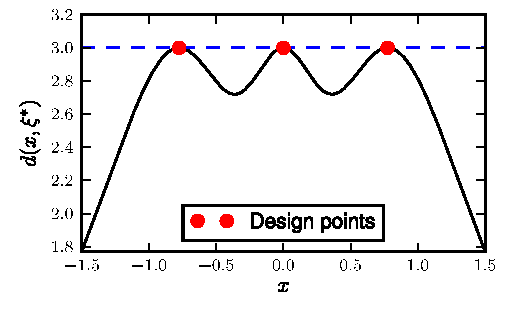
\includegraphics[width=0.9\textwidth]{fig1.eps}
\end{figure}

\begin{figure}
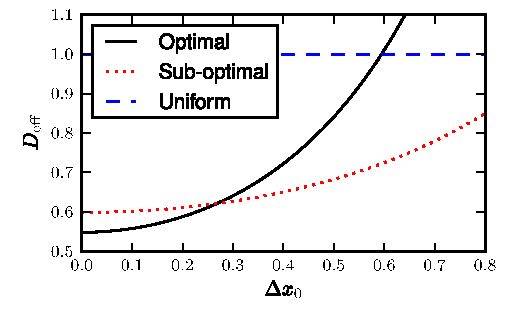
\includegraphics[width=0.9\textwidth]{fig2.eps}
\end{figure}

\begin{figure}
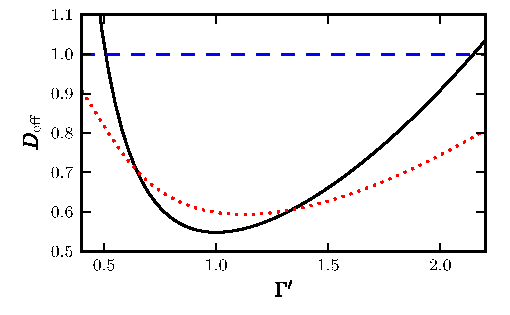
\includegraphics[width=0.9\textwidth]{fig3.eps}
\end{figure}

\begin{figure}
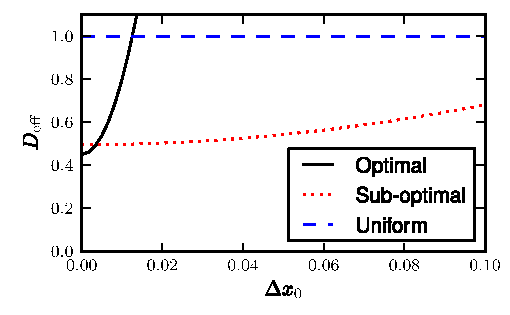
\includegraphics[width=0.9\textwidth]{fig4.eps}
\end{figure}

\section*{References}
\bibliographystyle{unsrt}
\bibliography{optimal}
\end{document}
